% \section{Control perfomance criteria}

% Como o objetivo deste trabalho é lidar com identificação e escolha de estruturas com o auxílio de estratégias VRFT, a serem aboradadas no capítulo \ref{cap:VRFT}, alguns conceitos necessários são apresentados nesta seção.
%
% Um elemento fundamental para projeto e análise de controladores na teoriade controle baseada em otimização, como é o caso do VRFT, é o conceito de \textit{desempenho de controle}. Na forma geral, este conceito pode ser expresso como a solução de um problema definido como
% \begin{equation}
%    \min_{\bm{\theta}} J(\bm{\theta}),
% \end{equation}
% onde $\vtheta \in \bm{R}$ é um vetor de $N$ parâmetros adotado como variável decisão e $J(\vtheta)$ é uma \textit{função de custo}\footnote{Outros termos também são conhecidos na literatura, como \textit{índice (ou função) de desempenho}, ou ainda, \textit{função objetivo}.}. Quanto menor o valor de $J$, melhor o desempenho segundo o critério adotado. Dependendo do objetivo de controle ou até mesmo por questões de garantias analíticas de estabilidade, diferentes funções de custo podem ser adotadas. Uma abordagem muito comum é escolher uma função de custo baseada na  norma-2 quadrática média\footnote{A norma-2 de um sinal discreto, ou vetor, $x(k)$ é definida como $||x(k)|| \triangleq \sqrt{ \sum_{k=1}^{N} [x(k)]^{2} }$. Elevando esse valor ao quadrado temos a norma-2 quadrática, que representa a energia do sinal que, dividida pelo número de amostras, como em \eqref{eq:H2}, resulta em sua energia média.}
% na forma
% \begin{equation}
%    ||x(k)||^{2} =\frac{1}{N}\sum_{k=1}^{N} \left[ x(k) \right]^{2} \triangleq \bar{\E} \left[ x(k) \right]^{2}
%    \label{eq:H2}
% \end{equation}
% em que $x(k)$ representa uma função genérica, $N$, o número de amostras e $\bar{\E}\left[ \cdot \right] $, um operador definido como
% \begin{equation}
%    \bar{\E}[x(k)] \triangleq \frac{1}{N}\sum_{k=1}^{N} [x(k)],
% \end{equation}
% que representa o cálculo da média amostral, e será usado no decorrer do texto em substituição ao somatório, por conveniência.
%
% O critério apresentado em \eqref{eq:H2} é conhecido como \textit{critério de desempenho} $H_2$ e é o que se adota neste trabalho e, para fins de objetividade, será o único abortado neste texto.
%
% O critério  $H_2$, para fins de controle, é definido de acordo com o objetivo de controle. Estes objetivos, em geral, são adotados como: (1) rastreamento de referência, (2) rejeição de ruídos e (3) economia de esforço de controle. Critérios mistos adotando mais de um destes objetivos, podem também ser definidos, como é o caso do (4) composite performance criteria. As próximas seções tratam destes critérios com um pouco mais de detalhes.

\section{Control System Setup and Notations}%
\label{sec:system_setup_}

% Nesta seção apresenta-se o sistema em malha fechada considerado, definindo as equações para seus componentes e introduzindo a notação utilizada ao longo do texto. Como pretende-se lidar com sistemas não lineares, adota-se a notação apresentada em \cite{campi2006}. Quando lidando com sistemas lineares, porém, esta notação pode parecer mais pesada que o necessário e uma notação mais usual pode ser adotada. Essas notações, são apresentadas no escopo do sistema de controle considerado e são detalhadas nas próximas subseções.
In this section, we present the closed-loop system considered, defining the equations for its components and introducing the notation used throughout the text. As it is intended to deal with non-linear systems, the notation presented in \cite{campi2006} is adopted. When dealing with linear systems, however, this notation may appear to be heavier than necessary and a more usual notation may be adopted. These notations are presented within the scope of the control system considered and are detailed in the next subsections.

\subsection{The control system}
\label{sub:o_sistema_de_controle}

% Considera-se um sistema de controle clássico do tipo SISO de um grau de liberdade, que pode ou não se encontrar sobre efeito de ruídos no sinal de saída. A Figura \ref{fig:diagrama_MF} apresenta o diagrama de blocos deste sistema, onde $C(q, \bm{\theta}, e)$ representa o Controlador, função do vetor de parâmetros $\bm{\theta}$ e $P(q,u)$, o modelo do processo, ou planta, que pode ser ou não conhecido. Os sinais $r(k)$,
It is considered a classic control system of the SISO type with a degree of freedom, which may or may not be under the effect of noise in the output signal. Figure \ref{fig:diagram_MF} shows the block diagram of this system, where $C(q, \bm{\theta}, e)$ represents the controller, a function of the vector of parameters $\bm{\theta}$ and $P(q,u)$, the process model, or plant, which may or may not be known. $r(k)$ 
\todo{Corrigir aqui. Usar somente P e C no diagrama e corrigir neste parágrafo} 
% $u(k)$, $\nu(t)$, $e(k)$, $y(k)$, e $y_\nu(k)$ são, respectivamente, os sinais de referência, controle, ruído, erro rastreamento, saída do processo e, por último, saída com ruído (ou sinal medido).
 $u(k)$, $\nu(t)$, $e(k)$, $y(k)$, and $y_\nu(k)$ are, respectively, the reference, control, noise, tracking error, process output and, finally, noise output signals.

\begin{figure}[htpb] 
   \centering
   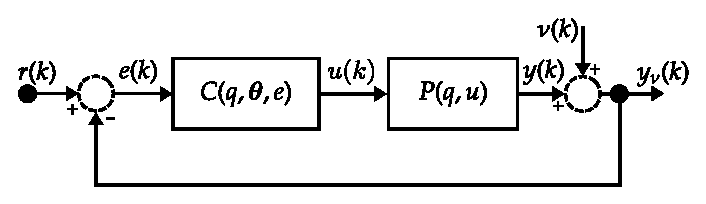
\includegraphics[width=0.8\textwidth]{Figs/diagrama_mf.eps}
   \todo[inline]{Mudar $e(k), u(k), y(k)$ e $y_{\nu}$, para $e_\theta(k), u_\theta(k), y_{\theta\nu}(k)$? Terei que mudar no texto também. Vide \ref{ass:noiseFree}.} 
   \caption{Sistema de controle.}
   \label{fig:diagrama_MF}
\end{figure}

\subsection{The process}%
\label{sec:TheProcess}

% O processo, ou planta, $P$ é um processo não-linear discreto no tempo do tipo SISO, com dinâmica não linear descrita como
The process, or plant, $P$ is a discrete non-linear time process of the SISO type, with nonlinear dynamics described as
\begin{equation}
   y(k)=p\left(y(k-1), \ldots, y(k-n_{P y}), u(k-1), \ldots, u(k-n_{P u})\right),
   \label{eq:yknl}
\end{equation}
% onde $p$ é uma função representando o processo, $n_{P y}$ é o máximo atraso na saída, $n_{P u}$ é o máximo atraso na entrada e $k$ o índice temporal.
where $p$ is a function representing the process, $n_{P y}$ is the maximum delay in the output, $n_{P u}$ is the maximum delay in the input and $k$ the temporal index.

% Por simplificação, é considerado que o atraso de tempo puro de $u$ para $y$ em $P$ é 1, mas o procedimento pode ser estendido sem problemas para atrasos maiores.
For simplicity, the pure time delay from $u$ to $y$ in $P$ is considered to be 1, but the procedure can be extended without problems for longer delays.

% Considera-se $P$ como um mapa não-linear que opera de $\mathbb{R}^{N}$ para $\mathbb{R}^{N}$. Quando sujeito às condições iniciais $i.c.= (y(0), \ldots, y(1-n_{P y}), u(-1), \ldots, u(1-n_{P u}) )$ e a um sinal de entrada no intervalo $[0, N-1]$ definido como $u(0{:}N-1) \triangleq [u(0) \cdots u(N-1)]^{T}$, $P$ gera uma saída dada por
  $P$ is considered a non-linear map that operates from $\mathbb{R}^{N}$ to $\mathbb{R}^{N}$. When subject to the initial conditions $i.c.= (y(0), \ldots, y(1-n_{P y}), u(-1), \ldots, u(1-n_{P u}) )$ and an input signal in the range $[0, N-1]$, defined as $u(0{:}N-1) \triangleq [u(0) \cdots u(N-1)]^{T}$, $P$ generates an output given by
\begin{equation}
   y(1{:}N) = P[u(0{:}N-1), \text { i.c. }].
\label{eq:Pnl}
\end{equation}

The following hypotheses are adopted:
\begin{assum}[ Process smoothness ]\label{ass:psuave}
   % A função $p$ que representa o processo é suave.
   The function $p$ that represents the process is smooth.
\end{assum}
\begin{assum}[ Uniqueness of the solution ]\label{ass:invert}
   % Para quaisquer condições iniciais dadas, se $u_{1}(0{:}N-1) \neq u_{2}(0{:} N-1)$, então $P\left[u_{1}(0{:} N-1), i . c .\right] \neq P\left[u_{2}(0{:} N-1), i . c\right]$.
   For any initial conditions given, if
   $u_{1}(0{:}N-1) \neq u_{2}(0{:} N-1)$, so $P\left[u_{1}(0{:} N-1), i . c .\right] \neq P\left[u_{2}(0{:} N-1), i . c\right]$.
\end{assum}

% A hipótese~\ref{ass:psuave} garante a invertibilidade do mapa $P$. A invertibilidade de $P$ para um sinal de entrada definido no intervalo $\left[ 0{:}N-1 \right]$
% implica na invertibilidade do mapa em um intervalo $[0{:}T]$, com $T\le N-1$ \citep{campi2004}.
The Assumption~\ref{ass:psuave} guarantees the invertibility of the $P$ map. The invertibility of $P$ for an input signal defined in the range $\left[ 0{:}N-1 \right]$
implies in the invertibility of the map in a range $[0{:}T]$, with $T\le N-1$ \citep{campi2004}.
% COMTEMP \todo{Ref.\ aqui --olhar \citep{campi2006}.} 

% COMTEMP \todo[inline]{Acabar aqui.} 

\subsection{The controller}%
\label{sub:o_controlador}

% O controlador considerado, assim como o processo, é representado por um modelo não-linear (que pode também ser linear). Para fins de identificação dos parâmetros pelo método VRFT, assunto abordado no capítulo \ref{cap:VRFT}, assume-se que uma estrutura (ou classe) é previamente escolhida. Este controlador pode ser descrito como
The controller considered, as well as the process, is represented by a non-linear model (which can also be linear). For the purpose of identifying the parameters by the VRFT method, subject addressed in the chapter \ref{cap:VRFT}, it is assumed that a structure (or class) is previously chosen. This controller can be described as
\begin{equation}
   u(k)=c\left(u(k-1), \ldots, u(k-n_{C u}), e(k), \ldots, e(k-n_{C e})\right),
\label{eq:uknl}
\end{equation}
% em que $n_{Cu}$ e $n_{Ce}$ são os máximos atrasos no sinal de controle (saída do controlador e no sinal de erro de rastreamento (entrada do controlador).
where $n_{Cu}$ and $n_{Ce}$ are the maximum delays in the control signal (controller output and tracking error signal (controller input).

% Assim como para o processo, o controlador é sujeito às condições iniciais $i.c.= u(-1), \ldots, u(-n_{C u}), e(-1), \ldots, e(-n_{C e})$
As for the process, the controller is subject to the initial conditions $$i.c.= u(-1), \ldots, u(-n_{C u}), e(-1), \ldots, e(-n_{C e})$$
% e quando alimentado com o sinal de erro $e(0{:}N-1)$, gera o sinal de controle $u(0{:}N-1)$, que é representado por
and when fed with the error signal $e(0{:}N-1)$, it generates the control signal $u(0{:}N-1)$, which is represented by
\begin{equation}
   u(0{:}N-1)=C[e(0{:}N-1), i.c.].
\label{eq:Cnl}
\end{equation}

% Neste trabalho, um dos objetivos é selecionar um controlador adequado dada uma classe fixa de controladores pelo método VRFT, conforme abordado no capítulo \ref{cap:VRFT}. Essa classe é formada por todos controladores parametrizados por
In this work, one of the objectives is to select a suitable controller given a fixed class of controllers by the VRFT method, as discussed in the chapter \ref{cap:VRFT}. This class is formed by all controllers parameterized by
\begin{equation}
   u(k)=c\left(u(k-1), \ldots, u(k-n_{C u}), e(k), \ldots, e(k-n_{C e}); \bm{\theta}\right),
\label{eq:uknl_par}
\end{equation}
% sendo $\bm{\theta} \in \mathbb{R}^{n_\theta}$ um vetor de $n_{\theta}$ parâmetros. O controlador parametrizado por $\bm{\theta}$ será aqui indicado por $C_{\theta}$, e o sinal de controle \eqref{eq:uknl} fica na forma
being $\bm{\theta} \in \mathbb{R}^{n_\theta}$ a vector of $n_{\theta}$ parameters. The controller parameterized by $\bm{\theta}$ will be indicated here by $C_{\theta}$, and the control signal \eqref{eq:uknl} is in the form
\begin{equation}
   u_{\theta}(0{:}N-1)=C_{\theta}[e(0{:}N-1), i.c.],
\label{eq:utheta}
\end{equation}
with
\begin{equation}
   e(0{:} N-1)\triangleq r(0{:} N-1)-y(0{:} N-1),
\label{eq:erro}
\end{equation}
representing the tracking error.

The following assumption is assumed for the controller:
\begin{assum}
   % O controlador $c(k)$ é uma função escalar \textit{suave} do vetor de parâmetros $\bm{\theta}$, de $u(k-1:k-n_{Cu})$  e de $e(k-0:k-n_{Ce})$, ou de forma simplificada
   % O controlador $c$ é representado por uma função escalar parametrizada como em \eqref{eq:uknl_par}, e assumido suave, ou de forma simplificada
   The $c$ controller is represented by a scalar function parameterized as in \eqref{eq:uknl_par}, and assumed to be smooth, or in a simplified way
   \begin{equation}
      c:\mathbb{R}^{n_{Cu}+n_{Ce}+1+n_{\theta}} \mapsto \mathbb{R} \text{ is smooth}.
      \label{eq:assumcon}
   \end{equation}
\end{assum}



\subsection{The feedback system}%
\label{sub:o_sistema_realimentado}

% As interconexões do sistema em malha fechada apresentado na Figura \ref{fig:diagrama_MF}, juntamente com as equações do processo \eqref{eq:Pnl} e do controlador \eqref{eq:Cnl} resultam na relação
The interconnections of the closed-loop system shown in Figure \ref{fig:diagrama_MF}, together with the equations of the process \eqref{eq:Pnl} and the controller \eqref{eq:Cnl} result in the relationship
\begin{align}
   y(1: N) &=P[u(0{:} N-1), i . c .] \nonumber \\
   &=P[C[e(0{:} N-1), i . c .], i . c .]
   \label{eq:CLSnl}
\end{align}

\subsection{Notation simplification}%
\label{sub:simplificações_nas_notações}

% Por simplificações nas notações, considera-se as condições iniciais da planta e do controlador nulas. Tal requerimento não é necessário, porém só leva  a complicações desnecessárias, principalmente na notação. Além do mais, se as N é grande o suficiente, as condições iniciais influenciam pouco para casos estáveis.
For simplifications in the notations, the initial conditions of the plant and the controller are considered null. Such a requirement is not necessary, but it only leads to unnecessary complications, especially in the notation. Furthermore, if the N is large enough, the initial conditions have little influence on stable cases.
% Além disso, os argumentos temporais são omitidos, resultando no uso dos símbolos: $u$ para representar $u(0{:}N-1)$, $r$ para $r(0{:}N-1)$, $e$ para $e(0{:}N-1)$ e  $y$ para $r(1{:}N)$. Note o avanço temporal de $y$ em relação às outras variáveis. Desta forma, representa-se  $y(0{:}N)$ é representado por $Dy$, sendo $D$ uma matriz nilpotente de deslocamento em atraso definida como
In addition, time arguments are omitted, resulting in the use of the symbols: $u$ to represent $u(0{:}N-1)$, $r$ for $r(0{:}N-1)$, $e$ for $e(0{:}N-1)$ and $y$ for $r(1{:}N)$. Note the time advance of $y$ in relation to the other variables. In this way, $y(0{:}N)$ is represented by $Dy$, with $D$ being a nilpotent delay displacement matrix defined as
\begin{equation}
   D \triangleq \begin{bmatrix} 
      0 & 0 & \dots & 0 & 0 \\
      1 & 0 & \dots & 0 & 0 \\
      0 & 1 & \dots & 0 & 0 \\
      \vdots & \vdots & \ddots & \vdots & \vdots \\
      0 & 0 & \dots & 1 & 0 \\
   \end{bmatrix} 
\label{eq:}
\end{equation}

% Com isso, \eqref{eq:CLSnl} pode ser rescrita como
With that, \eqref{eq:CLSnl} can be written as
\begin{equation}
   y = P[C[r-Dy]]
   \label{eq:ymf}
\end{equation}
% Ou, utilizando o controlador parametrizado de \eqref{eq:utheta},
Or, using the  parametrized controller \eqref{eq:utheta},
\begin{equation}
   y_{\theta} = P[C_{\theta}[r-Dy_{\theta}]]
   \label{eq:ytheta}
\end{equation}


\subsection{The control objective}%
\label{sub:the_reference_model}

% Um elemento fundamental para projeto e análise de controladores na teoriade controle baseada em otimização, como é o caso do VRFT, é o conceito de \textit{desempenho de controle}. Na forma geral, este conceito pode ser expresso como a solução de um problema definido como
A fundamental element for controller design and analysis in optimization-based control theory, as is the case with VRFT, is the concept of \textit{control performance}. In general, this concept can be expressed as the solution to a problem defined as
\begin{equation}
   \min_{\bm{\theta}} J(\bm{\theta}),
\end{equation}
% onde $\vtheta \in \mathbb{R}$ é um vetor de $n_{\theta}$ parâmetros adotado como variável decisão e $J(\bm{\theta})$ é uma \textit{função de custo}\footnote{Outros termos também são conhecidos na literatura, como \textit{índice (ou função) de desempenho}, ou ainda, \textit{função objetivo}.}. Quanto menor o valor de $J(\bm{\theta})$, melhor o desempenho segundo algum critério adotado. Dependendo do objetivo de controle, ou até mesmo por questões de garantias analíticas de estabilidade, diferentes funções de custo podem ser adotadas. Uma abordagem muito comum é escolher uma função de custo baseada na  norma-2 quadrática média\footnote{A norma-2 de um sinal discreto, ou vetor, $x(t)$ é definida como $||x(t)|| \triangleq \sqrt{ \sum_{t=1}^{N} [x(t)]^{2} }$. Elevando esse valor ao quadrado temos a norma-2 quadrática, que representa a energia do sinal que, dividida pelo número de amostras, como em \eqref{eq:H2}, resulta em sua energia média.}
where $\vtheta \in \mathbb{R}$ is a vector of $n_{\theta}$ parameters adopted as a decision variable and $J(\bm{\theta})$ is a \textit{cost function}\footnote{Other terms are also known in the literature, such as \textit{performance index (or function)}, or else, \textit{objective function}.}. The lower the value of $J(\bm{\theta})$, the better the performance according to some adopted criterion. Depending on the control objective, or even for reasons of analytical stability guarantees, different cost functions can be adopted. A very common approach is to choose a cost function based on the mean quadratic norm-2 \footnote{The norm-2 of a discrete signal, or vector, $x(t)$ is defined as $||x(t)|| \triangleq \sqrt{ \sum_{t=1}^{N} [x(t)]^{2} }$. Raising this value squared we have the quadratic norm-2, which represents the energy of the signal which, divided by the number of samples, as in \eqref{eq:H2}, results in its average energy.}
in the form
\begin{equation}
   ||x(k)||^{2} =\frac{1}{N}\sum_{k=1}^{N} \left[ x(k) \right]^{2} \triangleq \bar{\E} \left[ x(k) \right]^{2}
   \label{eq:H2}
\end{equation}
% em que $x(k)$ representa uma função genérica, $N$, o número de amostras e $\bar{\E}\left[ \cdot \right] $, um operador definido como
where $x(k)$ represents a generic function, $N$, the number of samples and $\bar{\E}\left[ \cdot \right] $, an operator defined as
\begin{equation}
   \bar{\E}[x(k)] \triangleq \frac{1}{N}\sum_{k=1}^{N} [x(k)],
\end{equation}
% que representa o cálculo da média amostral, e será usado no decorrer do texto em substituição ao somatório, por conveniência.
which represents the calculation of the sample mean, and will be used throughout the text to replace the summation, for convenience.

% O critério apresentado em \eqref{eq:H2} é conhecido como \textit{critério de desempenho} $H_2$ e é o que se adota neste trabalho e, para fins de objetividade, será o único abortado neste texto.
The criterion presented in \eqref{eq:H2} is known as \textit{performance criterion} $H_2$.

% O critério  $H_2$, para fins de controle, é definido de acordo com o objetivo de controle. Estes objetivos, em geral, são adotados como: (1) rastreamento de referência, (2) rejeição de ruídos e (3) economia de esforço de controle. Critérios mistos adotando mais de um destes objetivos, podem também ser definidos, como é o caso do (4) composite performance criteria. As próximas seções tratam destes critérios com um pouco mais de detalhes.
The $H_2$ criterion, for control purposes, is defined according to the control objective. These objectives, in general, are adopted as: (1) reference tracking, (2) noise rejection and (3) control effort saving. Mixed criteria adopting more than one of these objectives, can also be defined, as is the case of (4) composite performance criteria. The following sections deal with these criteria in a little more detail.


\subsubsection{The Reference Tracking Objective}%
\label{sub:the_reference_tracking_objective}
% Um dos principais objetivos do controle em malha fechada é fazer com que o sinal controlado siga um sinal de referência desejado, de modo que sejam o mais próximo possível. Desprezando-se o efeito do ruído na saída, e considerando um controlador parametrizado, a resposta do sistema em malha fechada é dada por \eqref{eq:ytheta}.
One of the main objectives of closed loop control is to make the controlled signal follow a desired reference signal, so that they are as close as possible. Disregarding the effect of noise on the output, and considering a parameterized controller, the response of the closed-loop system is given by \eqref{eq:ytheta}.

% Esse objetivo pode ser traduzido como a minimização de uma função custo dada pela norma-2 do erro de rastreamento, na forma
This objective can be translated as the minimization of a cost function given by 2-norm of the tracking error, in the form
\begin{equation}
   % J(\bm{\theta}) = \bar{\E}\left[ r(t) - y_r(t,\bm{\theta}) \right].
   J_r^N(\bm{\theta}) \triangleq || r - y_\theta ||^2 .
   \label{eq:Jr}
\end{equation}
% onde o operador $\bar{\E}\left[ \cdot \right] $ (operador de média amostral), é definido como
% \begin{equation}
% \bar{\E}[\cdot] \triangleq \frac{1}{N}\sum_{k=1}^{N} [\cdot]^{2},
% \end{equation}
% e será usado no decorrer do texto em substituição ao somatório por conveniência.

\subsubsection{The Reference Model Objective}%
\label{sub:The Reference Model Objective}

% Um fato bem conhecido na comunidade de controle é que na prática é impossível fazer com que a saída siga perfeitamente o sinal de referência durante todo o tempo, ou seja \eqref{eq:Jr} nunca será zero.
A well-known fact in the control community is that in practice it is impossible to make the output follow the reference signal perfectly at all times, that is, \eqref{eq:Jr} will never be zero.
% Para contornar esse fato uma saída é relaxar o objetivo de rastreamento por outro que satisfaça pré-requisitos desejados (como tempo de acomodação, instante de pico, sobressalto máximo, dentre outros), mas que seja menos exigente que a referência original.
To get around this fact, one way out is to relax the tracking objective by another that satisfies the desired prerequisites (such as accommodation time, peak time, maximum startle, among others), but which is less demanding than the original reference.

% Esse novo objetivo é traduzido para um modelo conhecido como \textit{modelo de referência} representado aqui por um mapa de $\mathbb{R}^{N}$ para $\mathbb{R}^{N}$, que mapeia um sinal de referência, digamos, $\tilde{r}$ para um sinal de saída $\tilde{y}$ com um comportamento desejado\footnote{o símbolo \ $\tilde{}$ \ enfatiza que estes sinais são para o modelo de referência.}.
This new objective is translated into a model known as \textit{reference model} represented here by a map from $\mathbb{R}^{N}$ to $\mathbb{R}^{N}$, which maps a reference signal, say, $\tilde{r}$ to an exit signal $\tilde{y}$ with a desired behavior \footnote{the symbol $\tilde{}$ emphasizes that these signals are for the reference model.}.
\begin{equation}
   M:\tilde{r} \in \mathbb{R}^N \mapsto \tilde{y} \in \mathbb{R}^N
\label{eq:Mmap}
\end{equation}
% Este mapa, a princípio pode ser um modelo não linear, desde que seja suave e invertível. Porém, em geral, por conveniência, é escolhido como um modelo linear, mas ainda sim deve ser invertível. Defini-se a seguinte hipótese:
This map, in principle, can be a non-linear model, as long as it is smooth and invertible. However, in general, for convenience, it is chosen as a linear model, but it must still be invertible. The following Assumption was defined:
\begin{assum}[Invertibility of the reference model]
   $M$ is lower triangular and invertible.
\end{assum}
% O fato de $M$ ser adotado como triangular inferior garante que será causal, com atraso puro maior ou igual a 1.
The fact that $M$ is adopted as a lower triangular ensures that it will be causal, with a pure delay greater than or equal to 1.
% Um exemplo de escolha típica para $M$, para o caso linear, é o filtro
An example of a typical choice for $M$, for the linear case, is the filter
\begin{equation}
   M(q)=\frac{b_{1} q^{-1}+\cdots+b_{n_{M r}} q^{-n_{M r}}}{1+a_{1} q^{-1}+\cdots+a_{n_{M y}} q^{-n_{M y}}}
\label{eq:Mq}
\end{equation}
% sendo $n_{Mr}$ e $n_{My}$ os máximos atrasos pra a referência e para a saída, respectivamente, e $q$ um operador de atraso. No domínio do tempo, \eqref{eq:Mq} corresponde a
where $n_{Mr}$ and $n_{My}$ are the maximum delays for the reference and for the output, respectively, and $q$ is a delay operator. In the time domain, \eqref{eq:Mq} corresponds to
\begin{align}
   \label{eq:ytMr}
   \tilde{y}(k)=-a_{1} \tilde{y}(k-1)-\cdots &-a_{n_{M y}} \tilde{y}\left(k-n_{M y}\right) +b_{1} \tilde{r}(k-1)+\cdots+b_{n_{M r}} \tilde{r}\left(k-n_{M r}\right)
\end{align}

% Uma vez definido o modelo de referência que traduz o comportamento desejado em malha fechada, o novo objetivo de controle é traduzido como
Once the reference model that reflects the desired behavior in closed loop has been defined, the new control objective is translated as

   % e será, neste texto, referido como $M(z)$, quando na forma de função de transferência (linear) ou $M(q)$ quando na forma de modelos temporais (linear ou não linear), ou simplesmente $M$ quando na forma apresentada na section \ref{sec:}. Neste sentido, uma nova função de custo é definida como
\begin{equation}
   J_{RM}^N(\bm{\theta}) \triangleq \left\lVert y_\theta - \tilde{y} \right\lVert^{2} = \left\lVert P[C_\theta[\tilde{r}-Dy_\theta]] - M[\tilde{r}] \right\lVert^{2}
   % J_{RM}^N(\bm{\theta}) \triangleq \bar{\E}\left[ y_r(k,\bm{\theta}) - y_{RM}(k) \right]^{2} = \bar{\E}\left[ T(q,\bm{\theta},r(k)) - M(q,r(k)) \right]^{2}
   \label{eq:Jy}
\end{equation}
% sendo $\tilde{y} = M[\tilde{r}]$ o sinal de saída do modelo de referência desejado, quando sobre efeito de um sinal de referência $r$. Tal critério é conhecido como \textit{critério do modelo de referência}.
 where $\tilde{y} = M[\tilde{r}]$ represents the output signal of the desired reference model, when under the effect of a reference signal $r$. This criterion is known as \textit{reference model criterion}.


\subsubsection{The Noise Rejection Objective}%
\label{sub:the_noise_rejection_objective}

% Outro objetivo comum em sistemas de controle é minimizar o efeito do ruído no sinal de saída. O sinal de saída devido somente a atuação do sinal de ruído no processo pode ser escrito como
Another common goal in control systems is to minimize the effect of noise on the output signal. The output signal due only to the action of the noise signal in the process can be written as
\begin{equation}
   y_{\theta\nu}(\bm{\theta}) \triangleq S_\theta[\nu] = \nu-P[C_\theta[Dy_{\theta\nu}],
\end{equation}
% em que $\nu \triangleq \nu(0{:}N)$ representa o sinal de ruído e $S_{\theta}$ um mapa de ruído para a saída do processo, ou seja $M:\nu \mapsto y_{\theta\nu}$, que, para o caso linear, é também conhecido como função sensibilidade. Quando analisada a magnitude deste sinal em função de alguma norma, tem-se o critério de desempenho de rejeição de ruído $J_\nu^N(\bm{\theta})$ que, utilizando a norma-2, é dado por
where $\nu \triangleq \nu(0{:}N)$ represents the noise signal and $S_{\theta}$ a noise map for the process output, i.e. $M:\nu \mapsto y_{\theta\nu}$, which, for the linear case, is also known as the sensitivity function. When analyzing the magnitude of this signal as a function of some norm, results in the performance criterion of noise rejection $J_\nu^N(\bm{\theta})$ which, using the 2-norm, is given by
\begin{equation}
   J_\nu^N(\bm{\theta}) \triangleq \norm{ y_{\theta\nu} }^2 = \norm{ S_\theta[\nu] }^2.
   \label{eq:Jnoise}
\end{equation}

% Assim como no caso do rastreamento, não é possível a eliminação completa do efeito do ruído e um relaxamento neste critério é desejável, pelos mesmos motivos. Neste caso é definida uma função sensibilidade desejada $S_{M}$\footnote{O índice $M$ é utilizado para manter a analogia com o índice utilizado pelo modelo de referência para o caso de rastreamento.} e adota-se o critério
As in the case of tracking, it is not possible to completely eliminate the effect of noise and relaxation in this criterion is desirable, for the same reasons. In this case, a desired sensitivity function is defined $S_{M}$ \footnote{The $M$ index is used to maintain the analogy with the index used by the reference model for the tracking case.}, and the following criterion is adopted
\begin{equation}
   J_{RM\nu}^N(\bm{\theta}) \triangleq  \norm{S_\theta[\nu] - S_M[\nu]}^{2}.
   \label{eq:JeRM}
\end{equation}





\subsubsection{The Economy of Control Effort Objective}%
\label{sub:the_economy_of_control_effot_objective}

% Um objetivo comum no projeto de controladores, principalmente na área de controle ótimo, é a minimização do esforço de controle. Para minimizar o sinal de controle o seguinte índice pode ser definido:
A common objective in the design of controllers, especially in the area of optimal control, is to minimize the control effort by means of control signal. To minimize the control signal, the following index can be defined:
\begin{equation}
   J_u^N(\bm{\theta}) \triangleq \norm{ u(k) }^{2},
   \label{eq:Ju}
\end{equation}
% sendo $u(k)$ o sinal de controle. Porém este índice não deve ser usado sozinho, uma vez que $J_u^N(\bm{\theta}) = 0$ implicaria em $u \equiv 0$. Portanto o que se faz é utilizar-se de uma combinação deste índice, com outros, por exemplo, com o objetivo de rastreamento de referência, resultando em
 where $u(k)$ is the control signal. However, this index should not be used alone, since $J_u^N(\bm{\theta}) = 0$ would imply $u \equiv 0$. So what is done is to use a combination of this index, with others, for example, with the reference tracking, resulting in
\begin{equation}
   J_\lambda^N = J_{RM}^N(\bm{\theta}) + \lambda J_u^N(\bm{\theta}),
   \label{eq:Jl}
\end{equation}
% em que $\lambda \in \mathbb{R}$ representa um parâmetro de ajuste.
where $\lambda \in \mathbb{R}$ represents an adjustment parameter.
% Ao se utilizar de controladores baseados em modelo de referência, como o caso do VRFT a ser visto no \ref{cap:VRFT}, um efeito de economia de esforço de controle pode ser obtido ao se escolher um modelo de referência adequado. Portanto, neste trabalho a inclusão do índice \eqref{eq:Ju} na função de custo é desconsiderado.
When using controllers based on a reference model, such as the case of VRFT (to be seen in \ref{cap:VRFT}), a control effort saving effect can be obtained by choosing an appropriate reference model. Therefore, in this work, the inclusion of the \eqref{eq:Ju} index in the cost function is disregarded.


\subsubsection{The Composite Performance Objective}%
\label{sub:the_composite_performance_objective}

% Outro objetivo, mais realista que o de rastreamento de referência, é o \textit{composite performance}, que objetiva tanto reduzir o erro de rastreamento quanto rejeitar efeitos do ruído na saída. Este critério é dado por
Another objective, more realistic than that of reference tracking, is \textit{composite performance}, which aims to both, reduce tracking errors, and reject noise effects on the output. This criterion is given by
\begin{equation}
   J_T^N(\bm{\theta}) \triangleq \norm{ y_{\theta\nu} - \tilde{y} }^2,
   \label{eq:JT}
\end{equation}
% em que, diferentemente de $\tilde{y}$ em \eqref{eq:Jy}, o sinal $y_{\theta\nu}= P[C_\theta[r-y_\theta]] + S[\nu]$ depende do ruído. O critério final será a soma dos dois critérios anteriores, uma vez que a referência e o ruído são sinais independentes estatisticamente e pode ser escrito como
where, unlike $\tilde{y}$ in \eqref{eq:Jy}, the signal $y_{\theta\nu}= P[C_\theta[r-y_\theta]] + S[\nu]$ depends on the noise. The final criterion will be the sum of the two previous criteria, since the reference and the noise are statistically independent signals and can be written as

\begin{equation}
   J_T^N(\bm{\theta}) = \norm{ P[C_\theta[r-Dy_\theta]] - M[r] }^{2} + \norm{ S[\nu] }^2.
   \label{eq:}
\end{equation}






\section{The Ideal Controller}%
\label{sec:ideal_controller}
% COMTEMP \todo{Tirar o ``Matched Control??''.}

% Considerando o sistema realimentado apresentado em \eqref{eq:ymf}, e assumindo a invertibilidade de $P$ e que $M$ é triangular inferior, resolvendo \eqref{eq:ymf} para $C$, é possível calcular o controlador ideal, que resulta nos parâmetros ótimos para $C_\theta$, desde que $C_\theta$ tenha mesma estrutura (ou pertença à mesma classe) do controlador ideal. Este controlador ideal é definido como:
Considering the feedback system presented in \eqref{eq:ymf}, and assuming the invertibility of $P$ and that $P$ is lower triangular, solving \eqref{eq:ymf} for $C$, it is possible to calculate the ideal controller, which results in the optimal parameters for $C_\theta$, as long as $C_\theta$ has the same structure (or belongs to the same class) as the ideal controller. This ideal controller is defined as:
\begin{equation}
   C_0 \triangleq P^{-1}(I-MD)^{-1}M,
\label{eq:}
\end{equation}
% onde $I$ é a matriz identidade e $C^{i}$ é o controlador ideal.
where $I$ is the identity matrix and $C^{i}$ is the ideal controller.

% Quando o $C_0$ é usado na malha fechada, o mapa de $r$ para $y$ é dado por $M$, ou seja, $y=M[r]$
When $C_0$ is used in the closed loop, the map from $r$ to $y$ is given by $M$, that is, $y=M[r]$

% Para o caso linear SISO (Single Input Single Output), se o modelo do processo é conhecido e considerando que este é de
For the linear SISO case, if the process model is known and considering that it is of
% \todo{[DONE] Falar aqui (citar) do trabalho da Lucíola no sentido de lidar com fase não mínima. Talvez citar Stogestad também.}
minimum phase, the ideal controller xxxxx can be written in the form of a transfer function as
\begin{equation}
   C_0(z) = \frac{M(z)}{P(z)\left(1-M(z)\right)},
   \label{eq:Cdz}
\end{equation}
% em que $P(z)$ e $M(z)$ representam respectivamente as funções de transferência do processo e do modelo de referência.
where $P(z)$ and $M(z)$, respectively, represent the transfer functions of the process and the reference model.

% Note que, se o processo é de fase não mínima, devido a zeros fora do círculo unitário no plano-$z$, a inversa de $P(z)$ em \eqref{eq:Cdz} resulta em instabilidade do sistema. Soluções para este problema têm sido apresentadas há décadas para projetos MBC, como por exemplo regras para sintonia de PID, como a desenvolvida por \cite{skogestad2003}.
Note that, if the process is non-minimum phase, due to zeros outside the unit circle in the $z$-plane, the inverse of $P(z)$ in \eqref{eq:Cdz} results in system instability. Solutions to this problem have been presented for decades for MBC projects, such as rules for PID tuning, such as the one developed by \cite{skogestad2003}.
% Uma abordagem no mais recente, no âmbito do DDC, é apresentada por \cite{campestrini2011}.
An most recent approach, within the DDC scope, is presented by \cite{campestrini2011}.
% COMTEMP \todo{Colocar um pouco mais sobre esteartigo aqui.} 


% COMTEMP \todo[inline]{Colocar aqui a respeito do caso não linear, como em \cite[p. 19]{campi2006}, mas antes introduzir notação.}


